\section{Phương pháp đề xuất}
\subsection{Mô hình}
Sau khi chạy thực nghiệm và đánh giá các phương pháp gợi ý trên dữ liệu MOOCCubeX \cite{mooccubex}, nhóm đã chọn ra được phương pháp tốt nhất là mô hình KGAT (chi tiết kết quả trong Mục \ref{sec:ketqua}). Vì vậy, trong phần này, nhóm sẽ trình bày cách chuyển đổi từ input sang output của mô hình KGAT, còn phương pháp chuẩn bị dữ liệu sẽ được trình bày ở phần \ref{sec:chuanbivadulieu}.

\begin{figure}[ht]
    \centering
    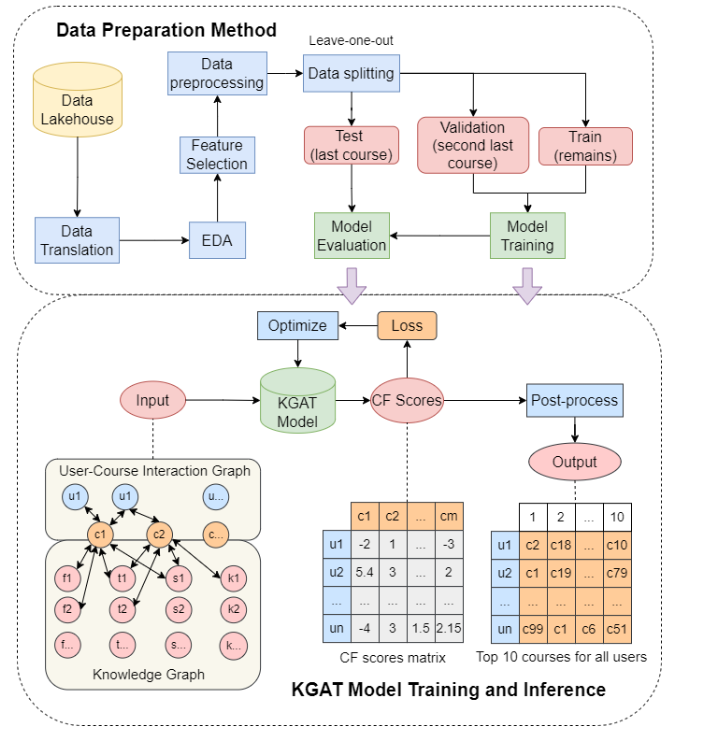
\includegraphics[width=0.9\textwidth]{figures/69.png}
    \caption{Hình minh họa quy trình thực nghiệm bài toán với cách tiếp cận sử dụng mô hình KGAT.}
    \label{fig:hinh4_1}
\end{figure}

Input của mô hình là collaborative knowledge graph chứa hai đồ thị thành phần như Hình \ref{}: user-item bipartite graph và knowledge graph. 
\begin{itemize}
    \item \textbf{User-item bipartite graph}: Biểu diễn mối quan hệ giữa người dùng và các khóa học đã đăng ký. 
    \item \textbf{Knowledge graph}: Biểu diễn mối quan hệ giữa khóa học và các thuộc tính của nó. Với node xuất phát là khóa học, đồ thị này bao gồm 4 loại quan hệ chính:
    \begin{itemize}
        \item Khóa học có khái niệm (concept) nào.
        \item Khóa học thuộc lĩnh vực (field) nào.
        \item Khóa học được dạy bởi giáo viên (teacher) nào.
        \item Khóa học được tổ chức bởi trường (school) nào.
        \item Khóa học có phần mô tả tương đồng với (course) nào.
    \end{itemize}
    Tính cả chiều ngược lại, tổng cộng có 8 loại quan hệ giữa khóa học và các thuộc tính.
\end{itemize}

Khi nhận được input, mô hình trả về một ma trận collaborative scores $cf\_scores \in \mathbb{R}^{n_{users} \times n_{courses}}$, với mỗi phần tử $cf\_scores_{i,j} \in \mathbb{R}$ ($i,j \in \mathbb{N}; 0 \leq i < n_{users}; 0 \leq j < n_{courses}$) cho biết mức độ phù hợp giữa user $i$ và khóa học $j$. Giá trị càng lớn thì user $i$ càng phù hợp với khóa học $j$.

Giai đoạn hậu xử lý (Hình \ref{}) thực hiện các bước sau:
\begin{itemize}
    \item Gán giá trị âm vô cùng cho $cf\_scores[i,j]$ nếu user $i$ đã đăng ký khóa học $j$.
    \item Thực hiện \texttt{argsort} giảm dần theo chiều axis=1 để loại bỏ các khóa học đã được đăng ký.
    \item Lấy top-10 khóa học có điểm cao nhất ứng với mỗi user để làm output.
\end{itemize}

\begin{figure}[ht]
    \centering
    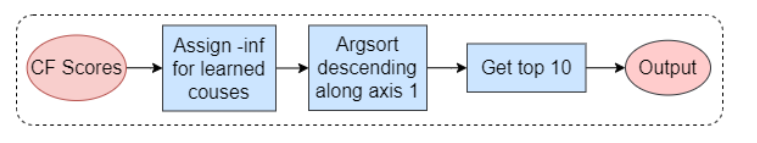
\includegraphics[width=0.9\textwidth]{figures/70.png}
    \caption{Hình minh họa giai đoạn hậu xử lý để lọc ra top-k khóa học được đề xuất.}
    \label{fig:hinh4_2}
\end{figure}


